\documentclass[11pt,a4paper]{article}
\usepackage[utf8]{inputenc}
\usepackage[german]{babel}
\usepackage[T1]{fontenc}
\usepackage{amsmath}
\usepackage{amsfonts}
\usepackage{float}
\usepackage{graphicx}
\usepackage[export]{adjustbox} %%used to change parameters in \includegraphics[scale=•]{•}
\usepackage{amssymb}
\usepackage[left=1cm,right=1cm,top=1cm,bottom=1cm]{geometry}
\usepackage{enumitem}
\usepackage{verbatim} %% Package to use \begin{comment}

\title{Geschäftsprozesse und Unternehmensmodellierung Zusammenfassung}
\author{Jonas Milkovits}

\setitemize{itemsep = 0.04cm} %% Globales Setzen des Parameters itemsep für itemize Tabellen (Package enumitem)

\graphicspath{{./files/}}

\begin{comment}

Copy-Paste-Area:

-------------------------------------------------------------------
Subsection mit Aufzählung:
\subsection{}

\begin{itemize}

\end{itemize}

-------------------------------------------------------------------
Aufführung über zwei Ebenen:

\item 
\item[] 
	\begin{itemize}
	\item 
	\item 
	\end{itemize}

-------------------------------------------------------------------
Bild mit Text daneben:

			\begin{minipage}{0.3\textwidth}
				\begin{figure}[H]
				\includegraphics[height=]{}
				\caption{}
				\end{figure}
			\end{minipage}
			\begin{minipage}[t]{0.5\textwidth}
				\vspace{cm}
				\begin{itemize}
				
				\end{itemize}
			\end{minipage}
-------------------------------------------------------------------
\end{comment}



\begin{document}

\maketitle
\tableofcontents
\pagebreak
 
\section{Einführung und Überblick} %% Vorlesung 1
\subsection{Geschäftsprozessanalyse}

\begin{itemize}
\item Entwicklung von Anwendungssystemen $\rightarrow$ Erfassung von Kundenanforderungen
\item IT- bzw. Prozessberatung $\rightarrow$ Ist-Analyse | Design | Implementierung 
\item Hilfreich zur Vereinheitlichung bei großen Transformationsprojekten
\end{itemize}

\subsection{Gesamtüberblick}

\begin{itemize}
\item Block 1: Prozess- und Unternehmensmodellierung
\item Block 2: Ansätze der Geschäftsprozessoptimierung
\item Block 3: Change Management, Analyse und Simulation
\end{itemize}

\section{Begriffe und Konzepte der Prozesmodellierung} %% Vorlesung 2
\subsection{Modelle und Modellierung}
\begin{itemize}


\item Was sind Modelle?
\item[] 
	\begin{itemize}
	
	\item Definition
		\begin{itemize}
		\item Beschränktes Abbild der Wirklichkeit
		\item Abbildung: Ein Modell ist stets ein Modell von etwas, das selbst wieder Modell sein kann
		\item Verkürzung: Modell erfasst nicht alle Attribute des Originals, sondern nur die die für Modellschaffer/-nutzer relevant sind
		\item Nutzung von Modellen um Problemlösungen zu finden, die am Original nicht möglich oder zu aufwendig gewesen wären
		\item Komplexitätsreduktion durch Abbildung der Realwelt in einem Modell
		\end{itemize}

	\item Modellarten:
		\begin{itemize}
		\item Ikonische, materiale Modelle (z.B.: Globus als Modell der Erde)
		\item Sprachlich-semantische Modelle (z.B.: Modell des Marktverhaltens)
		\item Isomorphe Abbildung (Jedem Element des Originals entspricht ein Element des Modells)
		\item Homomorphe Abbildung (Ausreichende Ähnlichkeit zwischen Original und Modell)
		\end{itemize}

	\item Modelltypen:
		\begin{itemize}
		\item Beschreibungsmodelle (deskriptiv)
		\item Erklärungsmodelle (Anwendung von Theorien auf Tatbestände)
		\item Entscheidungsmodelle (Einbau von Zielvorstellungen)
		\end{itemize}			
	
	\end{itemize}

\item Was ist Modellierung?
\item[] 
	\begin{itemize}
	\item Definiton:
		\begin{itemize}
		\item vereinfachende und zweckorientierte Abbildung eines Sachverhalts
		\item Abbildung sowohl als Verrichtung als auch als Ergebnis anzusehen
		\end{itemize}
	
	\item Ziel: Durch Konzentration auf die untersuchungsrelevanten Komponenten und ihrer Beziehungen die Transparenz eines Systems zu erhöhen
	\item Beispiel: Softwaremodellierung, Komplexitätsreduktion durch Zerlegung in verschiedene Teilmodelle
	\end{itemize}

\item Abgrenzung Prozess- und Unternehmensmodellierung
\item[] 
	\begin{itemize}
	\item Unternehmensmodell:
		\begin{itemize}
		\item Abbild der betrieblichen Realität
		\item idealtypischer Entwurf zur Planung eines betrieblichen Informationssystems
		\end{itemize}		 
		
	\item Unternehmensprozessmodell:
		\begin{itemize}
		\item Abbild der dynamischen Aspekte eines Informationssystems
		\item[$\Rightarrow$] Darstellung der Funktionen in ihrer zeitlich-logischen Abhängigkeit
		\item Ermöglicht Abbildung, Analyse und Optimierung betrieblicher Systeme und Prozesse
		\end{itemize}		 
	
	\end{itemize}

\end{itemize}

\subsection{Prozesse und Geschäftsprozesse}
\begin{itemize}

\item Warum (Geschäfts-)Prozessorientierung?
	\begin{itemize}
		\item Optimierung durch eventuellen Wechsel der Organisationsform (90 Grad Shift)	
		\item[] 
		\vspace{0.3cm}
			\begin{minipage}{0.3\textwidth}
				\begin{figure}[H]
				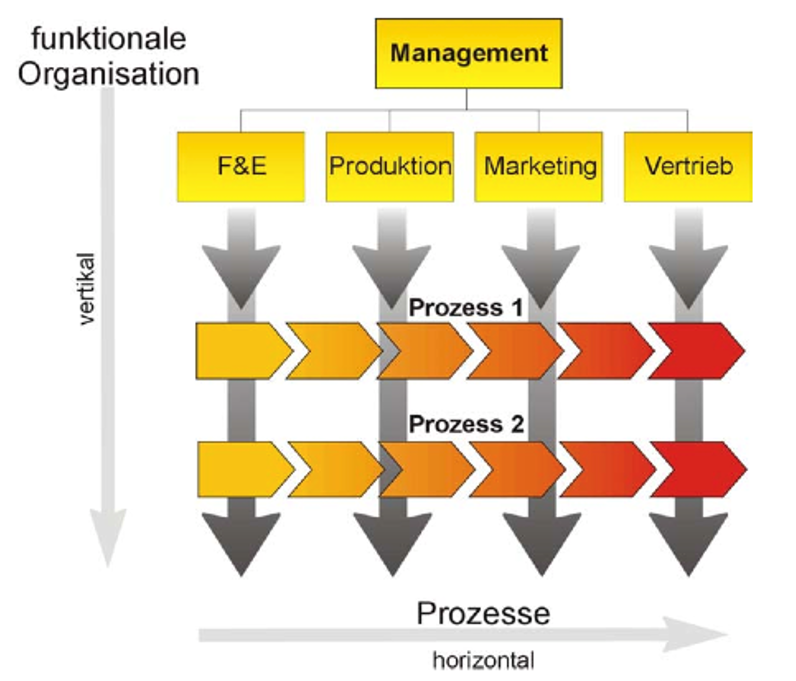
\includegraphics[height=5cm]{vertical_horizontal}
				\end{figure}
			\end{minipage}
			\begin{minipage}[t]{0.6\textwidth}
				\vspace{-3cm}
				\begin{itemize}
				\item Funktionsorganisation (vertikal)
					\begin{itemize}
					\item Spezialisierungsvorteile
					\item Starke Arbeitsteilung
					\item Vertikales Abteilungsdenken
					\item Fokus auf effizienter Fließbandarbeit
					\end{itemize}					 
				
				\item Prozessorganisation (horizontal)
					\begin{itemize}
					\item Kundenorientierung 
					\item Arbeitsintegration
					\item Guter Verlauf horizontaler Prozesse
					\item Fokus auf Kundenzufriedenheit/Produktivität
					\end{itemize}
				\end{itemize}
			\end{minipage}
			
	\end{itemize}
	\vspace{0.3cm}

\item Prozesse und deren Bestandteile
	\begin{itemize}
	\item Prozess: Folge von Schritten, die aus einer Reihe von Inputs einen Output erzeugen
	\item Geschäftsprozess: (Untermenge von betrieblichen Prozessen) 
		\begin{itemize}
		\item zielgerichtete, zeitlich-logische Abfolge von Aufgaben
		\item arbeitsteilige Ausführung durch mehrere Organisationseinheiten
		\item Wertschöpfende Aktivitäten, die von Kunden erwartete Leistung erzeugen
		\end{itemize}
	\item Klassifizierung:
		\begin{itemize}
		\item Nach Reichweite der Prozesse (unternehmens-, stellenübergreifend..)
		\item Nach Art des Objekt (materielle und immaterielle Prozesse)
		\item Nach Art der Tätigkeit (Support, Kern,..)
		\end{itemize}
	\item Charakterisierung (Strukturierung, Häufigkeit, Umfang, Dauer, Standardisierungsgrad)
	\end{itemize}

\item Geschäftsprozesse als eine Anwendungsform
	\begin{itemize}
	\item Prozessabstraktion:
	\item[] 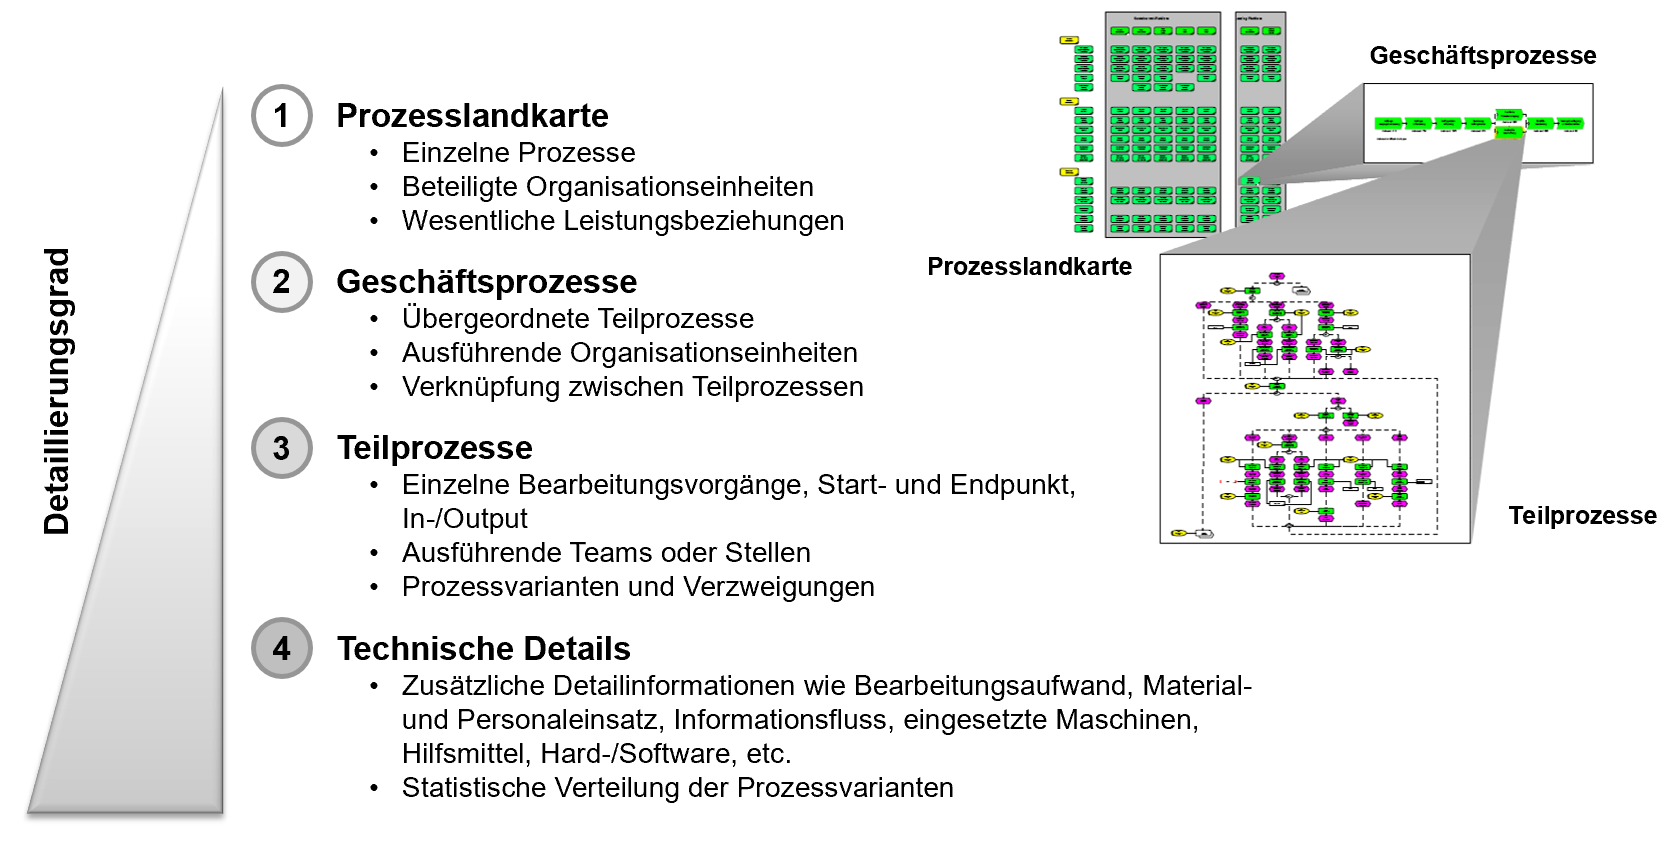
\includegraphics[width=0.8\textwidth]{prozessabstraktion}	
	\item Prozesslandkarte: Strukturierung von Prozessen / einzelne Prozesse in Wechselwirkungen
	\item Geschäfts-/Kernprozesse: Prozess mit hoher Wertschöpfung für den Kunden
	\item Unterstützungsprozess: Prozess mit geringer Wertschöpfgung für den Kunden 
	\item Steuerungsprozesse: Steuerung von Kern und Support anhand Unternehmenszielen
	\item Schnittstellen im Prozessablauf:
		\begin{itemize}
		\item Zuviele Schnittstellen führen zu Problemen
		\item Liegestelle, da zeitliche Abstimmungsprobleme bei Übergabe
		\item Irrtumsquelle, da Informationsverluste entstehene
		\item Quelle organisatorischer Unabhängikeit, Fehler schwer zurechenbar
		\item Barriere für Übertragung von Wissen
		\end{itemize}
	\end{itemize}
\end{itemize}

\section{ARIS (1) - Gesamtkonzept und EPK}
\subsection{Übersicht Prozessmodellierungsmethoden und das ARIS-Haus}
\begin{itemize}

	\item Übersicht zu formalen Methoden der Prozessmodellierung
		\begin{itemize}
		\item Skriptsprachen (Beschreibung mithilfe formaler Notation | hohe Präzision | geringe Anschaulichkeit)	
		\item Diagrammbasierte Methoden
			\begin{itemize}
			\item Datenflussorientierte Methoden
				\begin{itemize}
				\item Daten- und Informationsfluss zwischen Prozessen im Mittelpunkt
				\item Transformation des Datenflusses
				\item Beispiel: Datenflussdiagramm (SSA) (Modellierung von Arbeitsabläufen)
				\end{itemize}
			
			\item Objektorientierte Methoden
				\begin{itemize}
				\item Nutzung zur Softwareentwicklung
				\item Fachliche Beschreibung von funktionalen Anforderungen
				\item UML (Unified Modelling Language)
				\end{itemize}
				
			\item Kontrollflussorientierte Methoden
				\begin{itemize}
				\item Zeitlich logischer Ablauf von Aktivitäten, Funktionen im Fokus
				\item BPMN (Business Process Modeling and Notation) (Workflows)
				\item Ereignisgesteuerte Prozesskette (EPK) (Erstellung fachlicher Prozessmodelle zur Organisation)
				\end{itemize}							
			
			\end{itemize}				
		
		\end{itemize}
		
	\item Das ARIS-Modell
		\begin{itemize}
		\item Allgemeines
			\begin{itemize}
			\item ARIS = Architektur integrierter Informationssysteme
			\item Beschreibung von Unternehmen und Anwendungsoftware mit allen wesentlichen Merkmalen
			\item Modellierungsmethoden: z.B.: eEPK und WKD 
			\item Fokus auf Geschäftsprozess
			\end{itemize}
		
		\item ARIS-Sichten (House of Business Engineering
		\item[] \begin{minipage}{0.35\textwidth}
				\begin{figure}[H]
				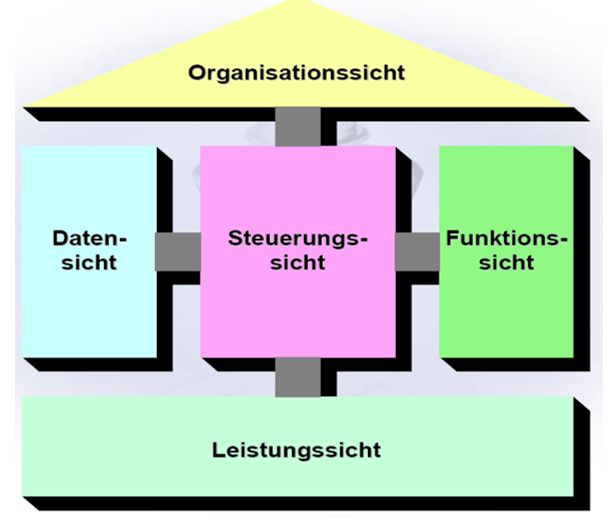
\includegraphics[height=6cm]{arishaus}
				
				\end{figure}
			\end{minipage}
			\begin{minipage}[t]{0.55\textwidth}
				\vspace{-1.5cm}
				\begin{itemize}
				\item Datensicht (Welche Informationen sind wichtig?)
				\item Funktionssicht (Welche Funktionen werden ausgeführt?)
				\item Organisationssicht (Welche Organisationseinheiten?)
				\item Leistungssicht (Welche Leistungen sind wichtig?)
				\item Steuerungssicht (Beziehung zwischen obigen)
				\end{itemize}
			\end{minipage}
			
		\pagebreak
			
		\item Das ARIS-Phasenmodell
			\begin{itemize}
			\item \textbf{1. Phase:} Betriebswirtschaftliche Problemstellung 
			\item[$\rightarrow$]  Grobe Tatbestände, nah an Zielen und fachlicher Sprachwelt orientiert
			\item \textbf{2. Phase:} Fachkonzept (Requirements Definition)
			\item[$\rightarrow$] Darstellung in formalisierter Beschreibungssprache
			\item \textbf{3. Phase:} DV-Konzept (Design Specification)
			\item[$\rightarrow$] Anpassung der Fachmodelle an die Anforderungen der Schnittstellen
			\item \textbf{4. Phase:} Technische Implementierung (Implementation Description)
			\item[$\rightarrow$] Übertragung des DV-Konzepts auf Komponenten (Hardware/Software)
			\end{itemize}
			
		\end{itemize}

\end{itemize}

\subsection{Wertschöpfungskettendiagramme}
	\begin{itemize}
	\item[] 
	\begin{figure}[H]
	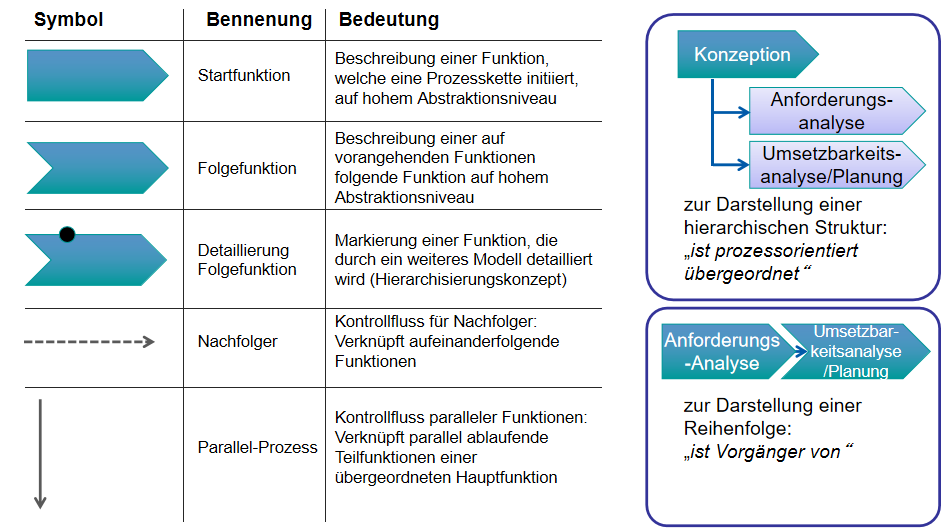
\includegraphics[width=18cm]{notationwkd} 
	\caption{Notation WKD}
	\end{figure}
	\item[] 
	\begin{figure}[H]
	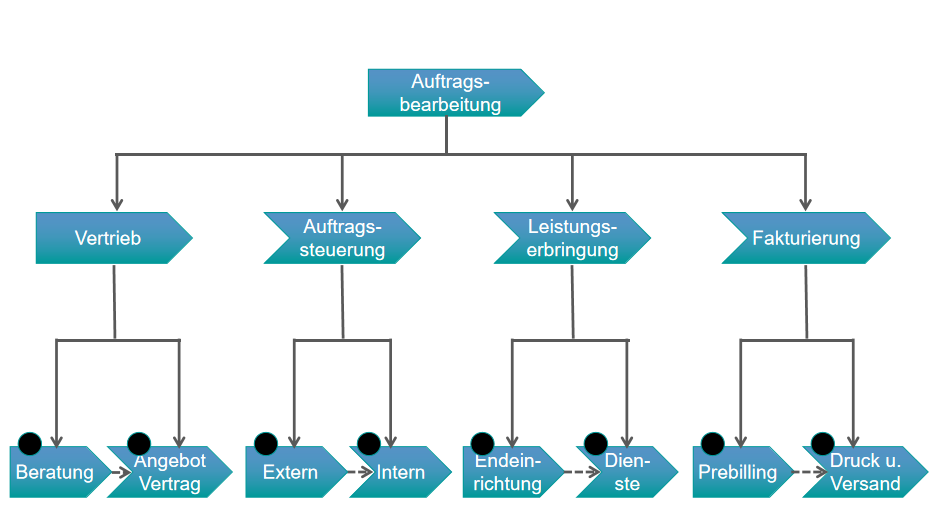
\includegraphics[height=8cm]{beispielwkd}
	\caption{Beispiel WKD}
	\end{figure}
	\end{itemize}

\subsection{Ereignisgesteuerte Prozessketten}
\begin{itemize}
	\item[]
			\begin{minipage}{0.15\textwidth}
				\begin{figure}[H]
				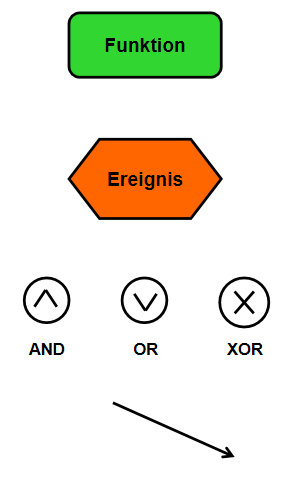
\includegraphics[height=5cm]{epkcomp}
				\end{figure}
			\end{minipage}
			\begin{minipage}[t]{0.75\textwidth}
				\vspace{-2.5cm}
				\begin{itemize}
				\item \textbf{Funktionen:} Verrichttungen oder Aktivitäten | Verbrauchen Zeit und Ressourcen
				\item[]
				\item \textbf{Ereignisse:} betriebswirtschaftlich relevante Zustände
				\item[]
				\item \textbf{Verknüpfungen:} Verbindung oder Trennung von Pfaden
				\item[]
				\item \textbf{Kanten:} Verküpfung der Objekte | Richtung relevant
				\end{itemize}
			\end{minipage}
	
	\item Verknüpfungen
		\begin{itemize}
			\item[] 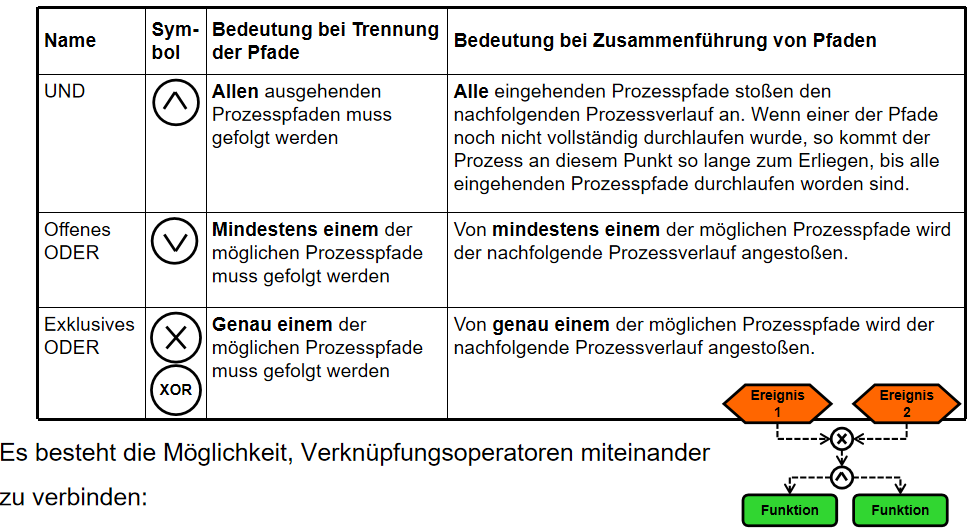
\includegraphics[width=16cm]{connec}
		\end{itemize}
		
	\item Modellierungsregeln
	 	\begin{itemize}
	 	\item Startet mit Ereignis
	 	\item Endet mit Ereignis
	 	\item Alternierende Folge von Ereignissen und Funktionen
	 	\item Maximal eine ausgehende und eine eingehende Kante
	 	\item Verküpfungen $\rightarrow$ Zusammenführen von Pfaden
	 	\item Beim Zusammenführen wieder selber Operator wie bei Verzweigung
	 	\item Nach einem einzelnen auslösenden Ereignis kein logischer Verknüpfungsoperator, der eine Entscheidung erforderlich macht (kein OR, 	
	 		  kein XOR)
	 	\item Entscheidungen werden immer in Funktionen getroffen
	 	\item[] 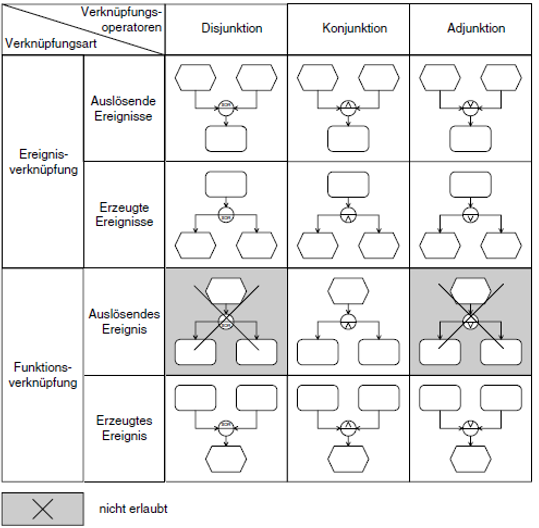
\includegraphics[height=5cm]{rulesaris}
	 	\end{itemize}
	 	
	 \item Modellierungsmuster
	 	\begin{itemize}
	 	\item Zerlegung von Ereignissen (OR)
	 	\item Parallele abläufe (AND)
	 	\item Alternative Abläufe (XOR)
	 	\end{itemize}
			
\end{itemize}

\subsection{Referenzmodelle}
\begin{itemize}

	\item Informationen
		\begin{itemize}
		\item Konkrete, abstrahierte Modelle
		\item Darstellung von techn. und betriebw. Fachinhalten bzgl. Strukturen und Abläufe
		\item gelten für eine Klasse von Objekten (höherer Abstraktionsgrad)
		\item Verwendung als Basis für Modellerstellung
		\item Induktive Enstehung aus KnowHow oder deduktiv aus theoretischen Erkenntnissen
		\item Abbildung über "best practice" oder "common practice"
		\item Erhöhung der Qualität eines Informationsmodells
		\item Beschleunigung des Prozesses der Modellerstellung
		\end{itemize}
	

\end{itemize}

\section{ARIS (2) - Modellierung erweiterter EPK}
\subsection{Erweiterte Ereignisgesteuerte Prozessketten}
\begin{itemize}
	\item Sichtenkonzept (Reduktion Komplexität bei Prozessmodellierung)
		\begin{itemize}
		\item Unterscheidung nach Prozess- und Struktursichten
		\item Prozesssicht (Beteiligte Modellierungsobjekte aus ablauforientierter Sicht)
		\item Struktursicht (Struktur der Modellierungsobjekte)
		\item[] 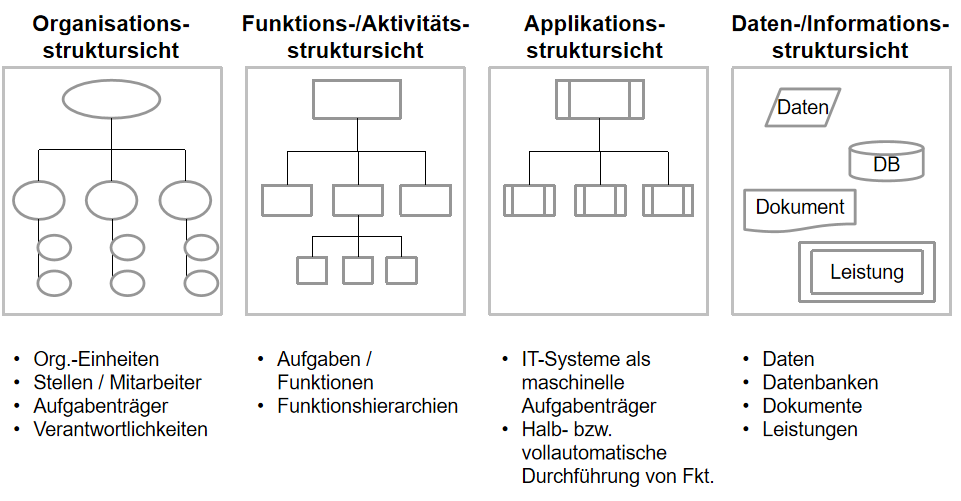
\includegraphics[width=15cm]{sichten}
		\end{itemize}
	
	\item Zusätzliche Komponenten einer eEPK
		\begin{itemize}
		\item \textbf{Organisationseinheiten, Stellen, konkrete Personen} (Träger der Funktionen)
		\item \textbf{Anwendungssysteme} (Software, untersützt Ausführung der Funktionen, Speichern der Daten)
		\item \textbf{Daten} (Input und Output von Funktionen, Dokumente als Datenträger)
		\item \textbf{Leistungen} (Ergebnis von Prozessketten, z.T. identisch mit Dokumenten)
		\item \textbf{Kantentypen} (Verschiedene Bedeutung)
		\item[] 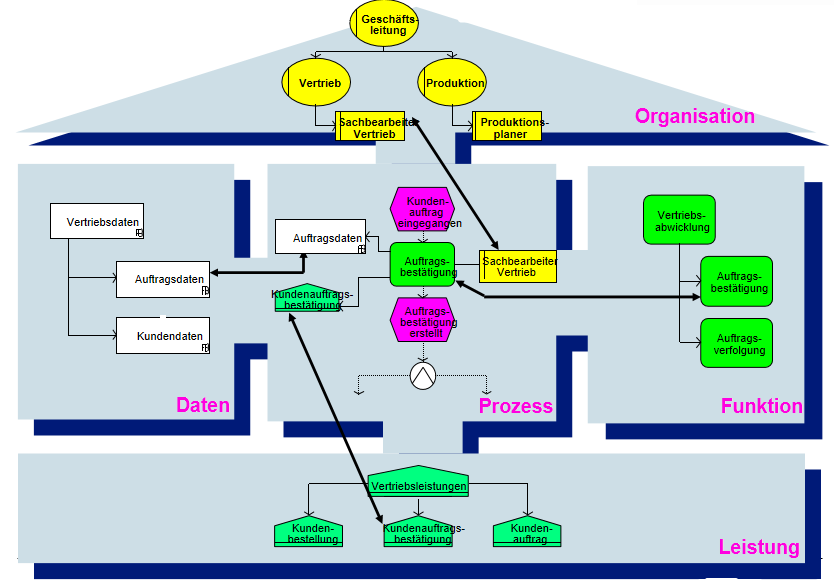
\includegraphics[width=15cm]{ariseepk}
		\end{itemize}


\end{itemize}

\subsection{Modellierung ergänzender Sichten}
\begin{itemize}
	\item Beispiel:
		\begin{itemize}
		\item[] 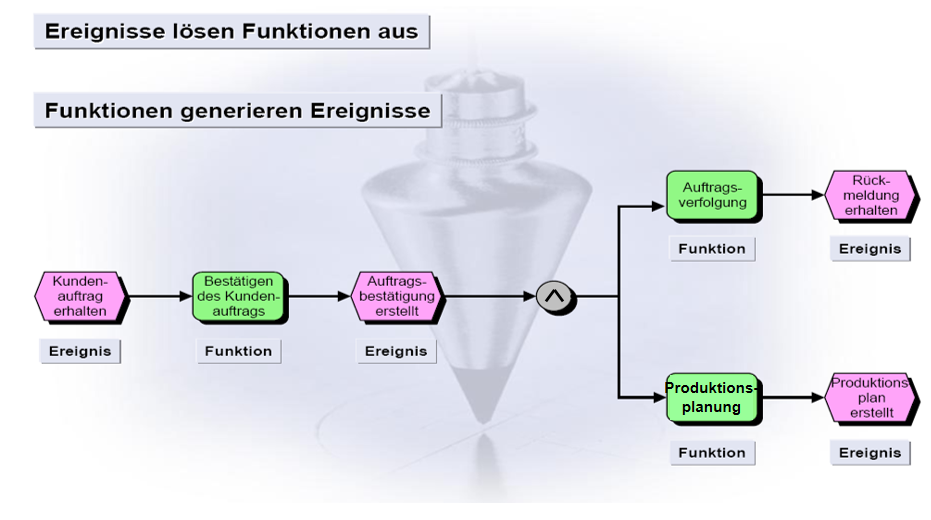
\includegraphics[width=15cm]{eepk1}
		\item[] 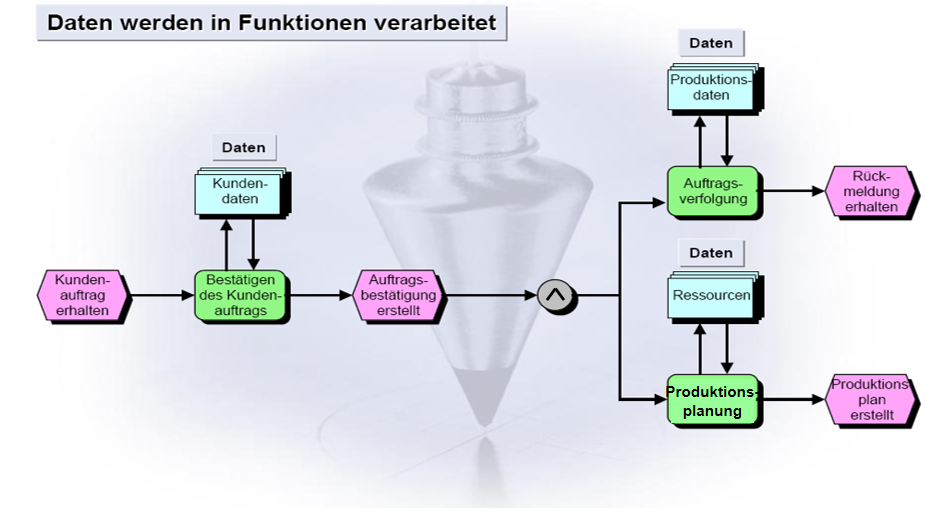
\includegraphics[width=15cm]{eepk2}
		\item[] 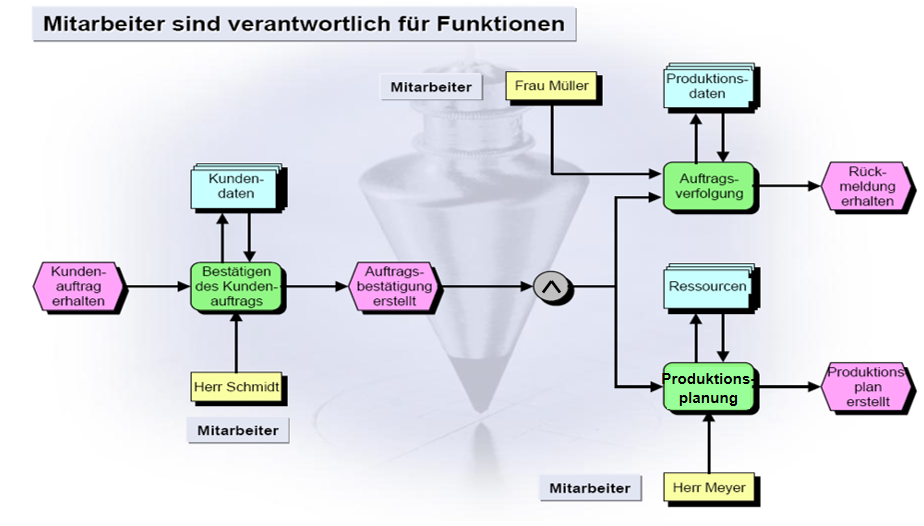
\includegraphics[width=15cm]{eepk3}
		\item[] 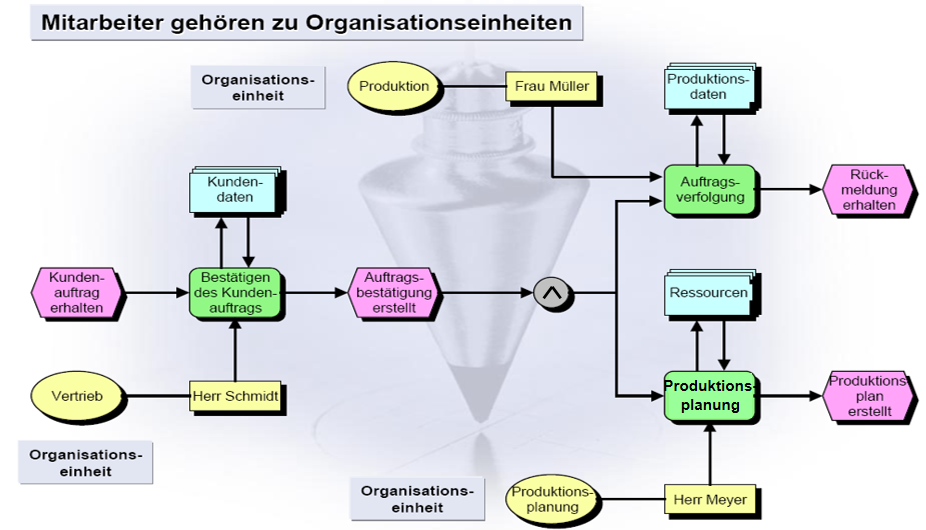
\includegraphics[width=15cm]{eepk4}
		\item[] 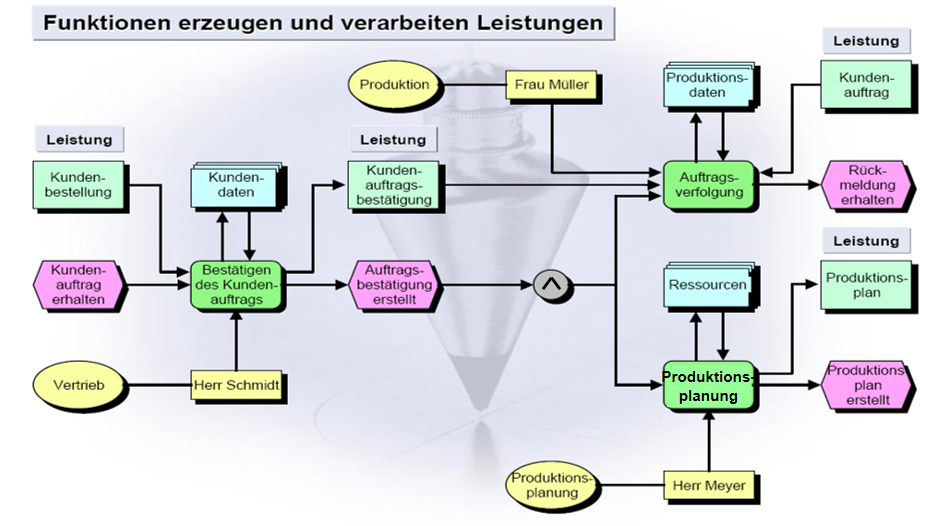
\includegraphics[width=15cm]{eepk5}
		
		\item[] 
			\begin{figure}[H]
			\centering
			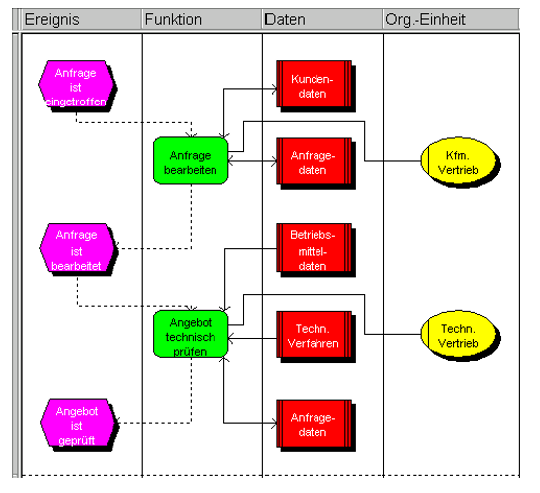
\includegraphics[width=15cm]{eepk6}
			\caption{Ereignis, Funktion, Daten und Organisationseinheiten als wesentliche Elemente}
			\end{figure}
		\end{itemize}
	
	\pagebreak
	
	\item \textbf{Funktionsbaum} (ARIS-Haus Funktionssicht)
		\begin{itemize}
		\item Funktion: Träger von Zeiten und Kosten | fachliche Aufgabe
		\item Darstellung des hierarchischen Aufbaus von Funktionen
		\item Zerlegung von Funktionen in Unterfunktionen
		\item[] 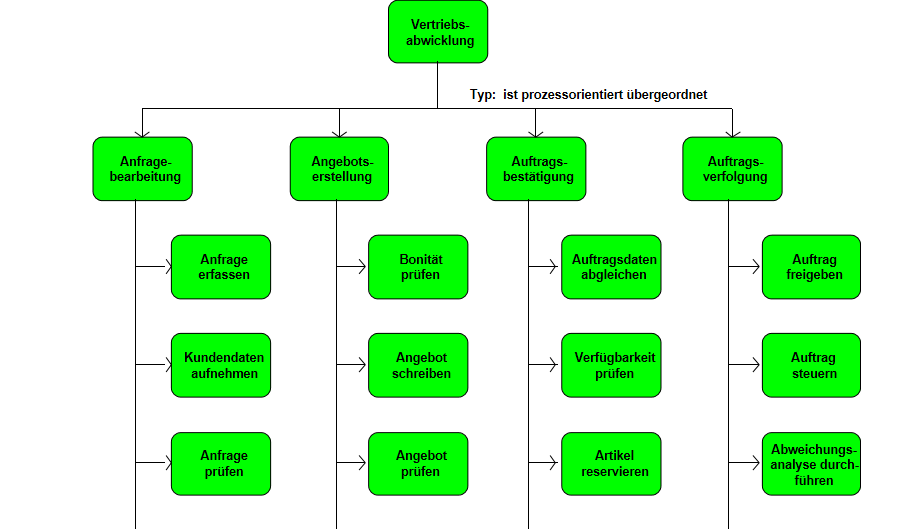
\includegraphics[width=15cm]{funktionen}
		\end{itemize}
		
	\item \textbf{Organigramm} (ARIS-Haus Organisationssicht)
		\begin{itemize}
		\item Darstellung der Aufbauorganisation eines Unternehmens
		\item Organisationseinheit: Träger der durchzuführenden Aufgaben (Teile der Gesamtaufgabe)
		\item[] 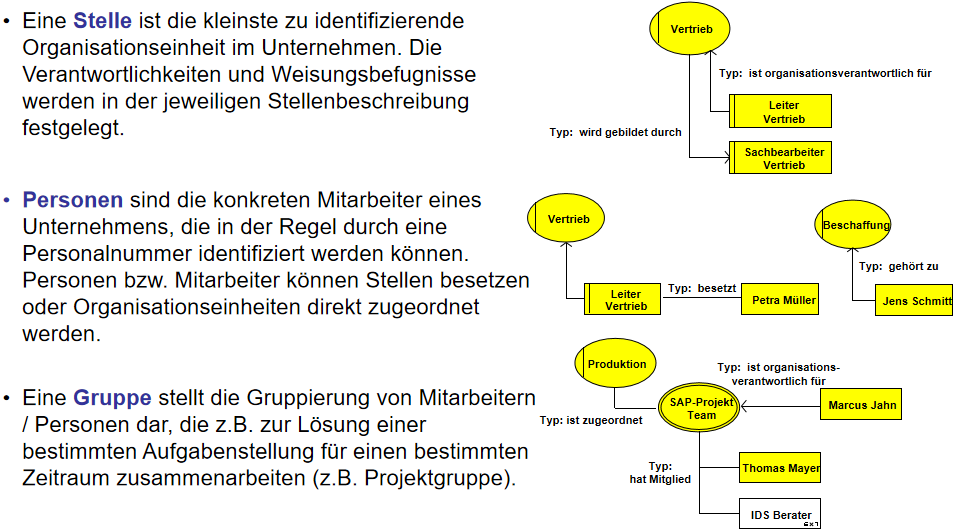
\includegraphics[width=15cm]{organi}
		\end{itemize}
	
	\pagebreak
	
	\item \textbf{Fachbegriffsmodel} (ARIS-Haus Datensicht)
		\begin{itemize}
		\item Beschreibt die unternehmensweit einheitlichen Begriff im Unternehmen
		\item Dient Kommunikation im Unternehmen
		\item[] 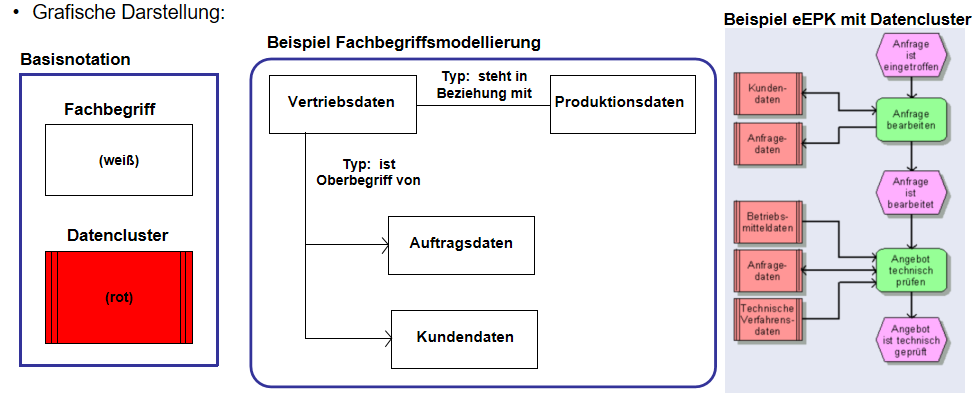
\includegraphics[width=15cm]{fachbegriffsmodell}
		\item ERM-Modell (Entity-Relationship-Modell)
		\item[] 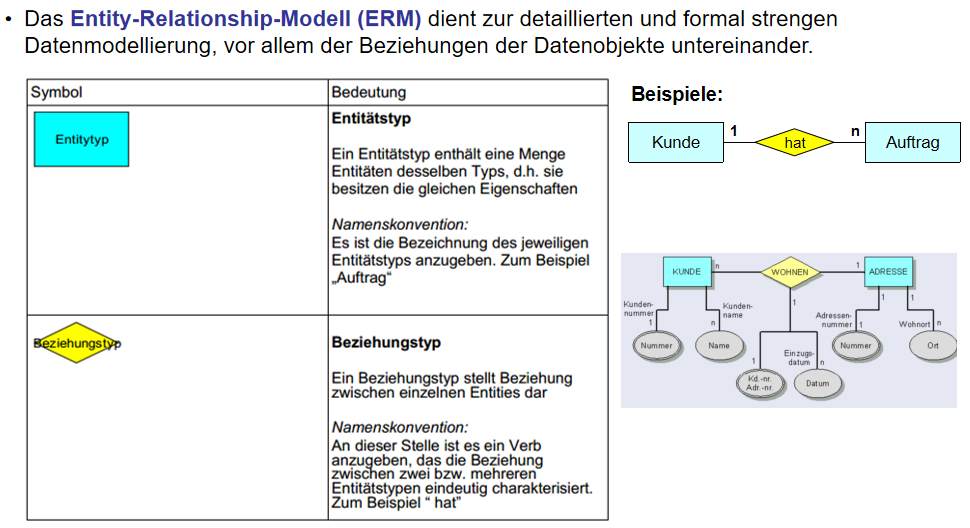
\includegraphics[width=15cm]{erm}
		\end{itemize}
\end{itemize}

\subsection{Grundsätze ordnungsgemäßer Modellierung (GoM) - Hintergrund}
\begin{itemize}
	
	\item Ordnungsrahmen (Unterstützung Klarheit, Qualität, Konsistenz)
	\item Ansprüche müssen vergleichbar sein
	\item[] 
	\begin{figure}[H]
	\centering
	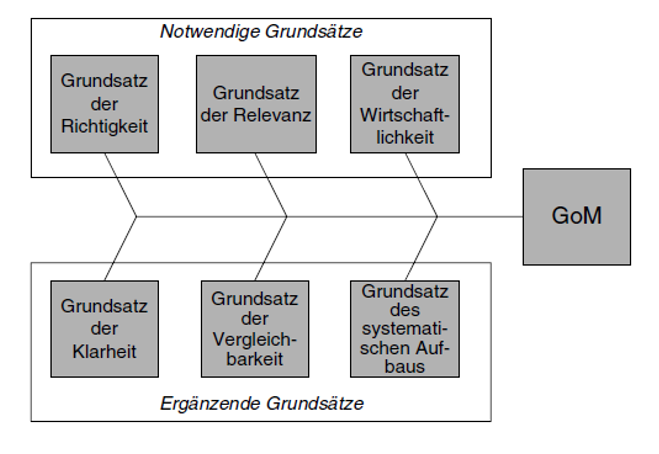
\includegraphics[width=9cm]{gom}
	\end{figure}	
	
	
\end{itemize}

\section{Geschäftsprozessmanagement}
\subsection{Motivation und begriffliche Grundlagen}

\begin{itemize}

\item Prozesse vs. funktionale Organisation
	\begin{itemize}
	\item Unternehmen als vernetzten System mit erbrachten Leistungen in Prozessen
	\item Zusätzliche Gliederung der Leistungsbringer in Organisationsstruktur
	\item Nachteile horizontaler Prozesse und vertikaler Strukturen:
		\begin{itemize}
		\item Vertikales Abteilungsdenken 
		\item Koordinationsprobleme bei übergreifenden Aufgaben
		\item Unzureichende Flexibilität
		\end{itemize}			
	\item Dysfunktionalitäten 
		\begin{itemize}
		\item Bearbeitungsfehler
		\item Doppelarbeiten
		\item Lange Durchlaufzeiten
		\end{itemize}			
		
	\end{itemize}
	
\item Prozessorganisation
	\begin{itemize}
	\item Definition: Strukturierung von organisatorischen Einheiten anhand von Kern-/Unterstützungsprozessen
	\item Unternehmensübergreifende Betrachtung
	\item Informationelle Vernetzung
	\item Ausgeprägte Kunden-/Marktsicht
	\end{itemize}
	
\item Geschäftsprozessmanagement
	\begin{itemize}
	\item Definition: integriertes Konzept von Führung, Organisation und Controlling
	\item[$\rightarrow$] Zielgerichtete Steuerung der Geschäftsprozesse
	\item Ausrichtung anhand der Bedürfnissen der Kunden und anderer Interessensgruppen
	\item Erhöhung der Effizienz und Effektivität
	\item Wesentliche Merkmale:
		\begin{itemize}
		\item Strategie- und kundenorientierte Definition der Geschäftsprozesse
		\item Multidimensionale Prozesssteuerung über Effektivitäts- und Effizienzparameter
		\item Prozessoptimierung durch Prozesserneuerung und Prozessverbesserung
		\end{itemize}
	\item Eigenschaften des Geschäftsprozessmanagement:
		\begin{itemize}
		\item Zielgerichtet (Unternehmensziele)
		\item Übergreifend (IT als auch Fachbereich)
		\item Proaktiv (zukünftige Entwicklungen)
		\item Integriert (Planungs- und Kontrollprozesse, aber auch Alltägliches)
		\item Methodisch
		\item Messbar durch Einsatz von Zielkennzahlen
		\end{itemize}			
	\end{itemize}
	
	
\end{itemize}

\subsection{Management von Geschäftsprozessen (5-Phasen Modell)}
\begin{itemize}
\item Identifizierung von Geschäftsprozessen
	\begin{itemize}
	\item Top-Down-Ansatz (Ausgehend von Geschäftsstrategie)
	\item Bottom-Up-Ansatz (Identifizierung der Prozessschritte auf unterster Ebene)
	\end{itemize}
	
\item Prozessbeschreibung
	\begin{itemize}
	\item SIPOC-Analyse (Supplier, Input, Process, Output, Customer..)
	\item EPK-Modelle
	\end{itemize}

\item Prozesscontrolling
	\begin{itemize}
	\item Prozessplanung, Prozesskontrolle, Informationsversorgung
	\item Soll/Ist-Vergleich von Messgrößen und Zielgrößen
	\end{itemize} 
	
\item Zielgrößen / Prozessleistungen
		\begin{itemize}
		\item Bsp.: Zeit-Kosten-Qualitäts-Dreieck
		\item Effektivitäts- und Effizienzüberlegungen
		\item Beispiele: Kundenzufriedenheit, Prozessqualität, Prozesskosten
		\item ''SMART''e Ziele:
			\begin{itemize}
			\item specific (eindeutig definiert)
			\item measurable (messbar)
			\item agreed to (Akzeptiert von Empfängern)
			\item realisitic (möglich)
			\item time bound (Terminvorgaben)
			\end{itemize}
		\item Zielgrößenbäume
		\end{itemize}

\item Verbesserung
	\begin{itemize}
	\item Abweichungsanalyse
	\item Ursachenanalyse
	\item Schwachstellenanalyse
	\item Korrektur bzw. Umgestaltungsmaßnahmen
	\item Neu- und Umgestaltung von Geschäftsprozessen
	\end{itemize}		

\end{itemize}


\section{Geschäftsprozessoptimierung}
\subsection{Grundlagen der Geschäftsprozessoptimierung}
\begin{itemize}
\item Allgemeine Ziele:
	\begin{itemize}
	\item Verringerung der Kosten zur Steigerung der Wettbewerbsfähigkeit
	\item Qualitative Verbesserung der Prozesse
	\item Nachhaltige Etablierung zeitlich beschleunigter Prozesse
	\end{itemize}
\item Prozesserneuerung zur Leistungssteigerung (\textbf{Revolution})
	\begin{itemize}
	\item Große Veränderungen in Ausnahmssituationen
	\item Hohe Chancen, aber auch Risiken
	\item Radikaler Umbruch
	\item[$\rightarrow$] Business Process Reengineering
	\end{itemize}

\item Prozessverbesserung zur Leistungssteigerung (\textbf{Evolution})
	\begin{itemize}
	\item Schrittweise, fortschreitende Verbesserungen
	\item Eher geringes Risiko
	\item permanente Aufgabe
	\item[$\rightarrow$] Kaizen und Lean Management
	\end{itemize}
\end{itemize}

\subsection{Ansätze zur Geschäftsprozessverbesserung}
\begin{itemize}
\item Kontinuierliche Prozessverbesserung - das Kai'Zen Konzept
	\begin{itemize}
	\item Kai = Veränderung
	\item Zen = zum Besseren
	\item Streben nach ständiger Verbesserung
	\item Grundlegende Verhaltensweise im Unternehmen, jeden Tag Verbesserungen
	\item ganzheitliche Optimierung
	\item Lean-Management entwickelte sich daraus
	\end{itemize}
	
\item Lean Managament
	\begin{itemize}
	\item Vermeidung von Veschwendung, von Variabilität und Inflexibilität, also jeglicher Art von Ineffizienz
	\item Fokus auf \textbf{Verschwendung}
		\begin{itemize}
		\item Wertschöpfende Tätigkeiten (Kunde ist bereit dafür zu bezahlen) $\rightarrow$ verbessern
		\item Verdeckte Wertschöpfung (ohne Wertschöpfung, aber erforderlich) $\Rightarrow$ verändern
		\item Offene Verschwendung (nicht notwendige Schritte) $\rightarrow$ abschaffen
		\item 7+1 Quellen der Verschwendung
		\vspace{0.3cm}
		\item[]	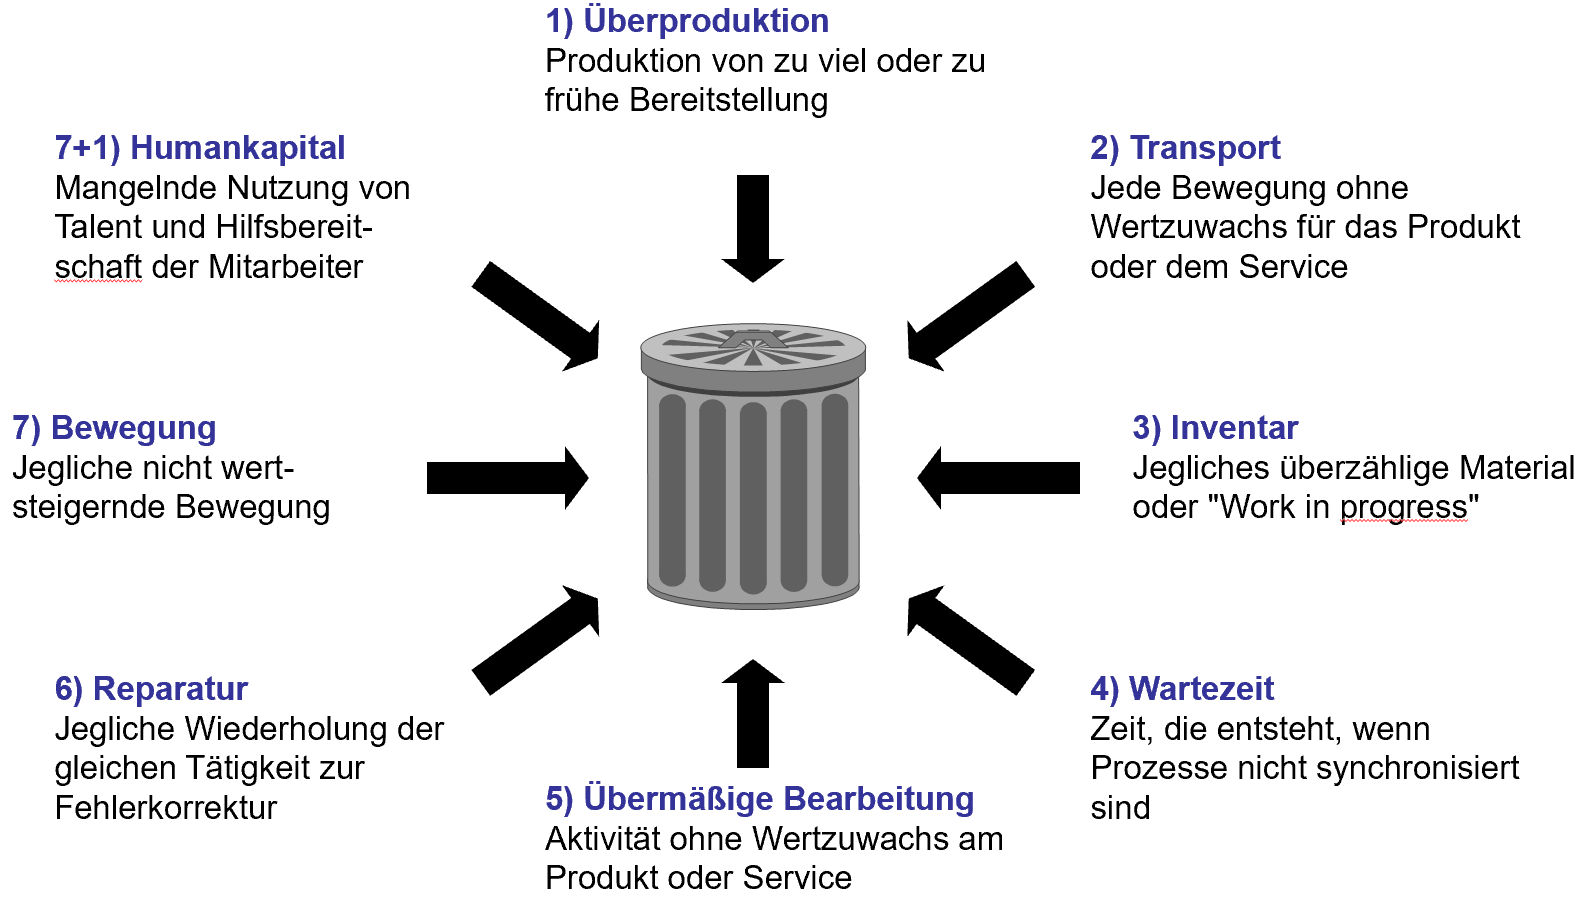
\includegraphics[width=15cm]{verschwendung}				
		\end{itemize}
	
	\item Fokus auf \textbf{Variabilität}
		\begin{itemize}
		\item Erhöhung der Kosten aufgrund von Sicherheits- bzw. Schadenskosten
		\item Schematische Analyse mithilfe von Ursache-Wirkungsdiagrammen
		\item Keep asking Why until you get to the root of the problem
		\item[$\rightarrow$] Angriff an Problemstellen
		\end{itemize}
		
	\item Fokus auf \textbf{Inflexibilität}
		\begin{itemize}
		\item Viele verschiedene Gesichtspunkte
		\item z.B. Anfrage: Bett in 1 Woche | Angebot: Bett in 6 Wochen
		\item[$\rightarrow$] Verlust des Preisaufschlags für schnelle Lieferung		
		
		\end{itemize}
	
	\end{itemize}
\end{itemize}

\subsection{Ansätze zur Geschäftsprozesserneuerung - Business Process Reengineering}
\begin{itemize}
\item Fundamentales Überdenken und radikale Redesign von Unternehmensprozessen
\item[$\rightarrow$] Verbesserung um Größenordnungen
\item Vorhergehensweise:
	\begin{itemize}
	\item Fundamental (Alles in Frage stellen, Erst Was und dann Wie)
	\item Radikal (Grundlegende Veränderungen, Völlig neue Wege)
	\item Dramatisch (Zerstörung des Alten und Aufbau von etwas Neuem
	\end{itemize}
\item Drei Ideen des Business Process Reengineering:
	\begin{itemize}
	\item Prozess-Idee
		\begin{itemize}
		\item 90 Grad Shift der Organisation (hin zu prozessorientiert)
		\item Einteilung in Kern- und Supportprozesse
		\item Reines Prozessmodell (Prozessteams/Prozess-Owner)
		\end{itemize}
		
	\item Triage-Idee (Segmentierung)	
		\begin{itemize}
		\item Funktionale Segmentierung (F\&E, Produktion, Vertrieb)
		\item Komplexität (Schwere Fälle, Einfache Fälle)
		\item Kundengruppen (z.B. bei Spezialwissen für Kundengruppen)
		\end{itemize}
		
	\item Informationelle Vernetzung (Potenziale der Informationstechnologie)
		\begin{itemize}
		\item Vollkommen neue Anwendungen / Dezentraler Zugriff
		\item Bsp.: Tele-Arbeit (verschiedene Standorte)
		\item Überwindung geographischer Distanzen
		\item Aufgabenintegration und -koordination verbessern
		\end{itemize}
	\end{itemize}
	
\item Vorteile
	\begin{itemize}
	\item ganzheitlicher Ansatz
	\item Kunde steht im Mittelpunkt
	\end{itemize}
	
\item Nachteile
	\begin{itemize}
	\item Eventuelle Zerstörung funktionaler Strukturen
	\item Oft Widerstand, da BPR zu Personalabbau führt
	\end{itemize}

\end{itemize}

\section{House of IT Functions and Change Management}
\subsection{House of IT Functions}
\begin{itemize}
\item IT-getriebener Ansatz
	\begin{itemize}
	\item Schnelle Suche nach IT-Lösung ohne Untersuchung des Problems im Detail
	\item keine optimale Lösung für operatives Geschäft
	\end{itemize}
	
\item Prozessorientierter Ansatz
	\begin{itemize}
	\item Nachhaltige Verbesserung durch IT-Systeme
	\item IT als Instrument der Prozessverbesserung
	\end{itemize}
	
\item[] 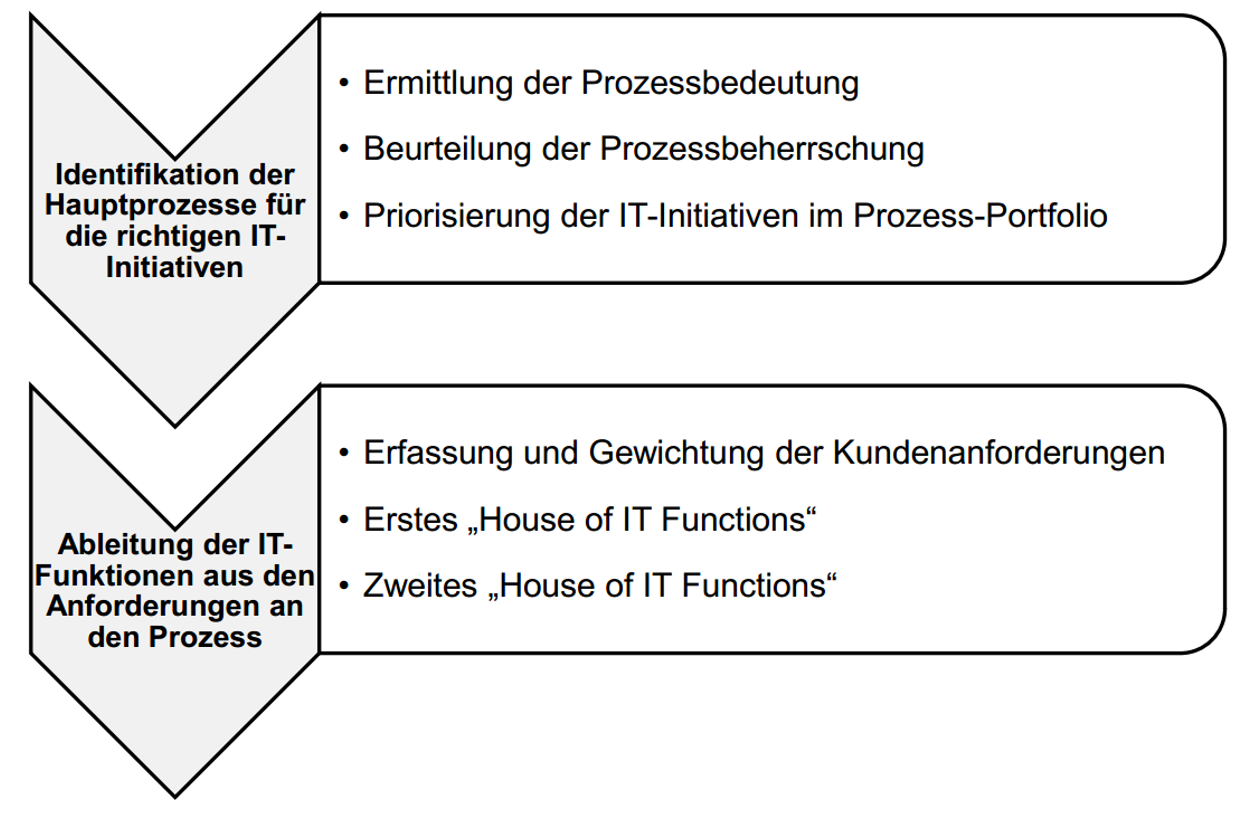
\includegraphics[width=15cm]{itprozess}

\item Zentrale Größen im House of IT-Functions
	\begin{itemize}
	\item Prozessbedeutung (Höhe der Ressourcenanbindung | Differenzierungspotential vom Wettbewerb)
	\item Prozessbeherrschung (Gleichbleibende Qualität, Zeit, Kosten)
	\item IT-Unterstützung (Durchdringungsgrad, Anwenderakzeptanz,..)
	\item Ziel: Prozessrangliste zur Analyse der strategischen Lenkung
	\end{itemize}

\item Methodischer Ansatz "House of IT-Functions"
	\begin{itemize}
	\item[] 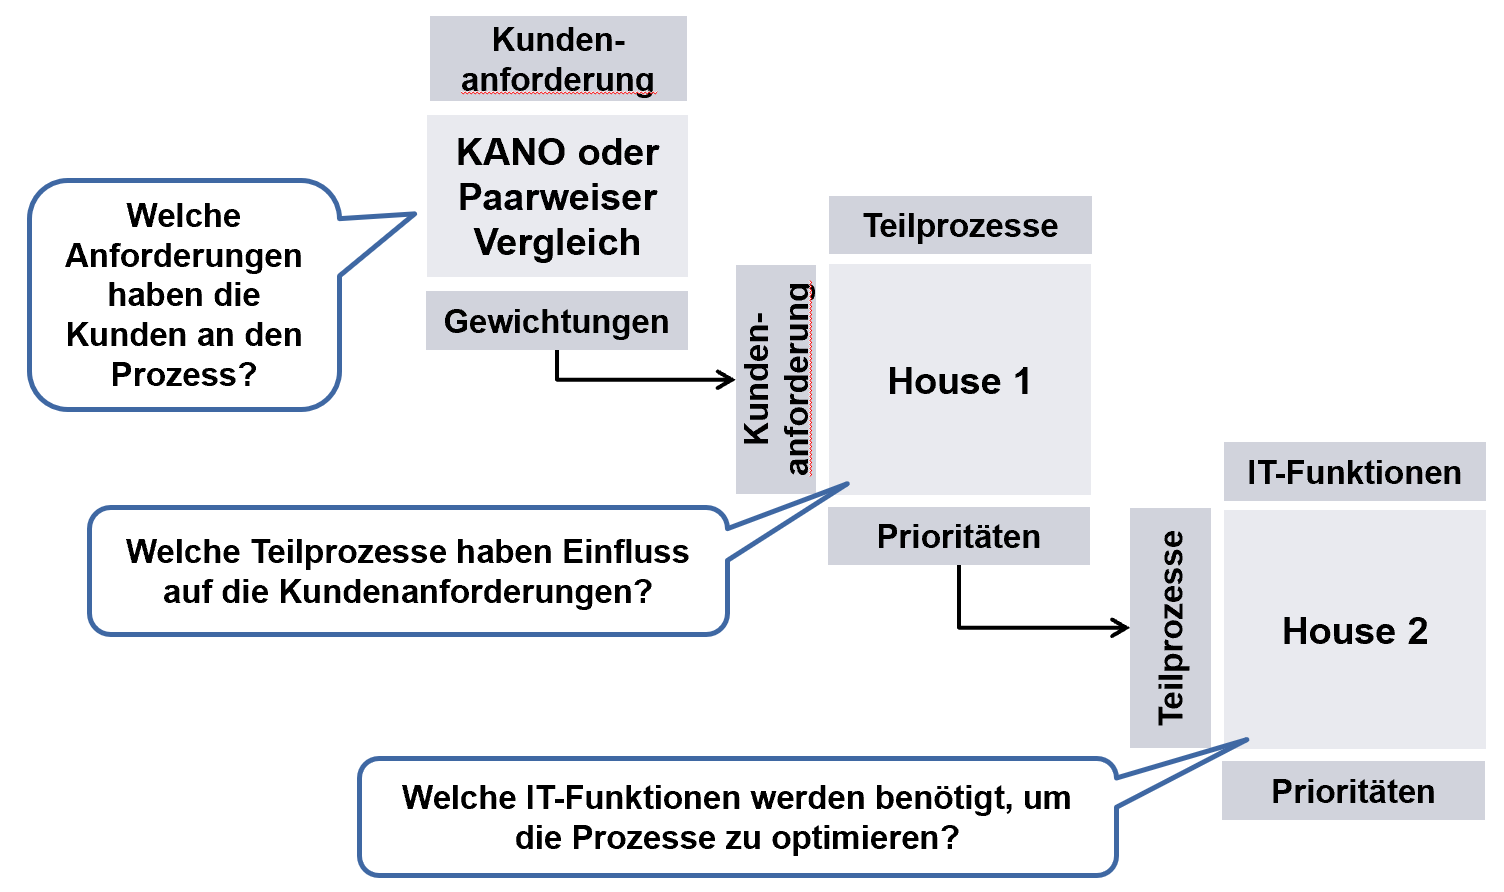
\includegraphics[width=15cm]{methodhouseofit}
	\end{itemize}
	\item Das erste "House of IT-Functions"
	\item[] 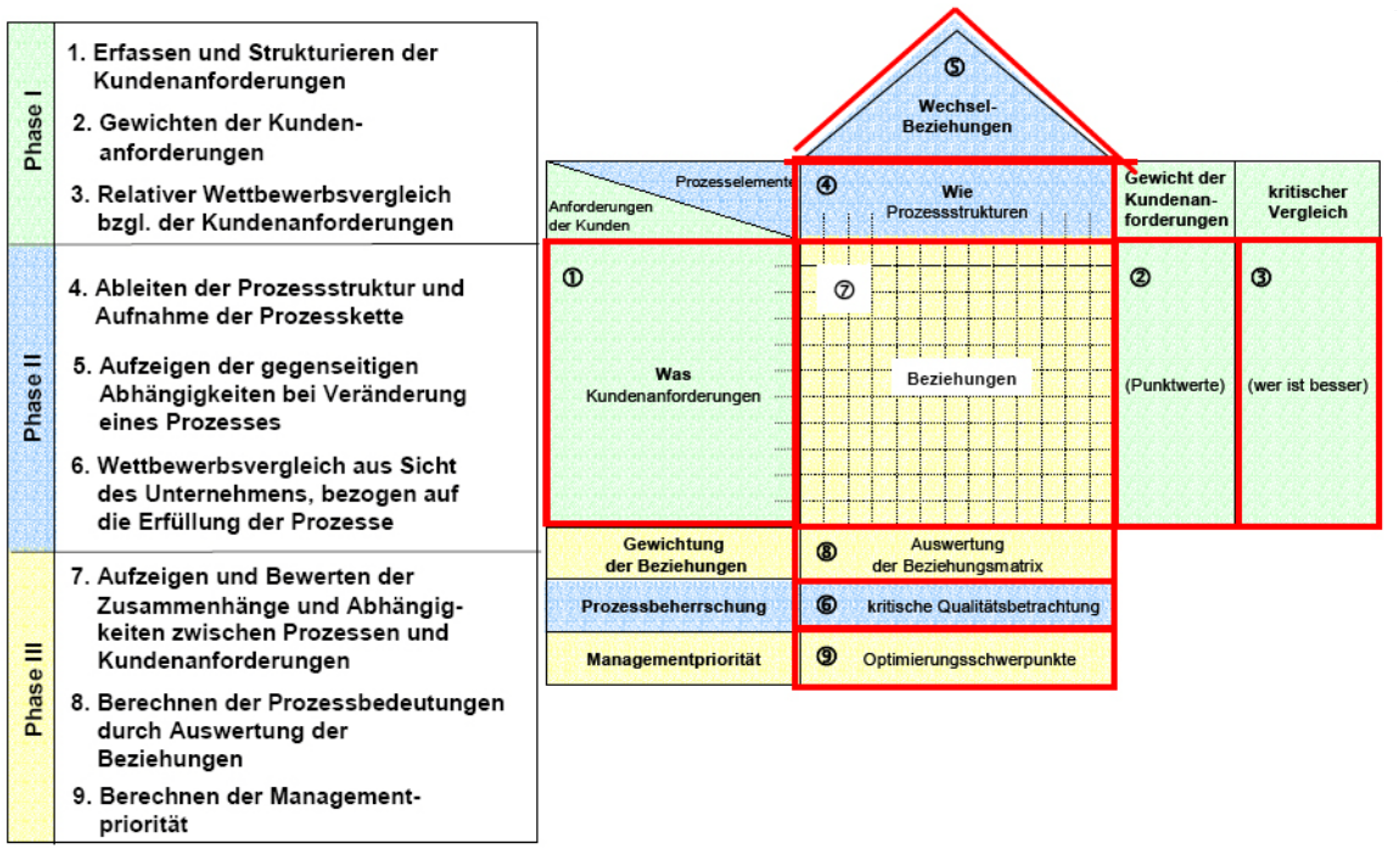
\includegraphics[width=17cm]{houseofit1}
		\begin{itemize}
		\item 1. Erfassung und Auswahl der Kundenanforderungen 
		\item[] (induktiv = direkt beim Kunden | deduktiv = Annahmen aufgrund von Erfahrungen)
		\item 2. Gewichtung der Kundenanforderungen (Kano-Modell)
		\item 3. Relativer Wettbewerbsvergleich der Kundenanforderungen
		\item[] Veränderung des Rangwertes aus SChritt 2 abhängig von Anforderungserfüllungsgrqd
		\item[] Optimierungsgewicht = Rangwert Schritt 2 - Erfüllungsgrad Schritt 3
		\item 4. Ableiten der Prozessstruktur und Aufnahme der Teilprozesse
		\item 5. Aufzeigen der gegenseitigen Abhängigkeiten bei Veränderung eines Prozesses
		\item[] Beachten der zusammenhängenden Prozesse
		\item 6. Wettbewerbsvergleich aus Sicht des Unternehmens (interne Unternehmenssicht)
		\item 7. Aufzeigen und Bewerten der Zusammenhänge und Abhängigkeiten zwischen Prozessen und Kundenanforderungen		
		\item[$\rightarrow$] Identifikation der für die Kunden wichtigen Teilprozesse
		\item 8. Berechnen der Prozessbedeutung durch Auswerten der Beziehungen
		\item[] Multiplikation Rangwert Schritt 3 mit Beziehungsstärke Schritt 7
		\item[] Anschließend Addition der Werte je Teilprozess
		\item 9. Berechnen der Managementpriorität
		\item[] 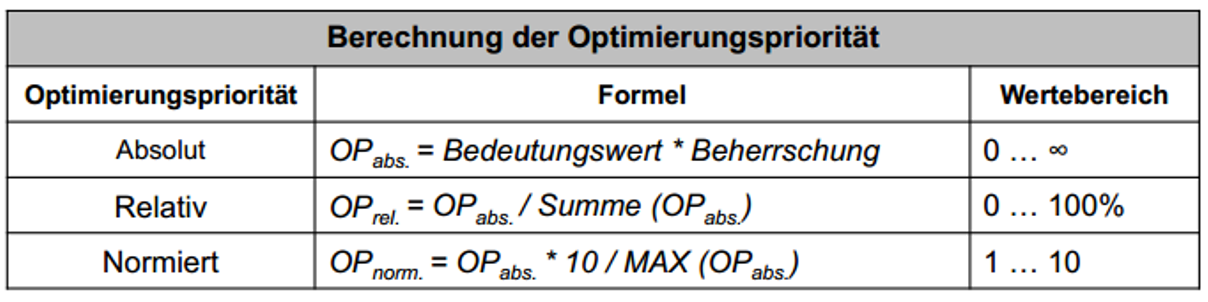
\includegraphics[width=10cm]{optiprio}
		
		\end{itemize}
	
	\item Das zweite "House of IT-Functions"
		\begin{itemize}
		\item Verknüpfung von IT-Funktionen und Prozessen (aus dem ersten Haus)
		\end{itemize}
		
\end{itemize}

\subsection{Change Management}
\begin{itemize}

\item Scheitern von BPR Projekten (meistens wegen Widerständen der Mitarbeiter)
\item Aktive Unterstützung von Mitarbeitern notwendig
\item[$\rightarrow$] Change Management
	\begin{itemize}
	\item Planung, Durchsetzung und Kontrolle von Veränderungen
	\item Optimale Ausgestaltung des Weges
	\item Die Feldtheorie Kurt Lewins
		\begin{itemize} \vspace{0.3cm}
		\item[] 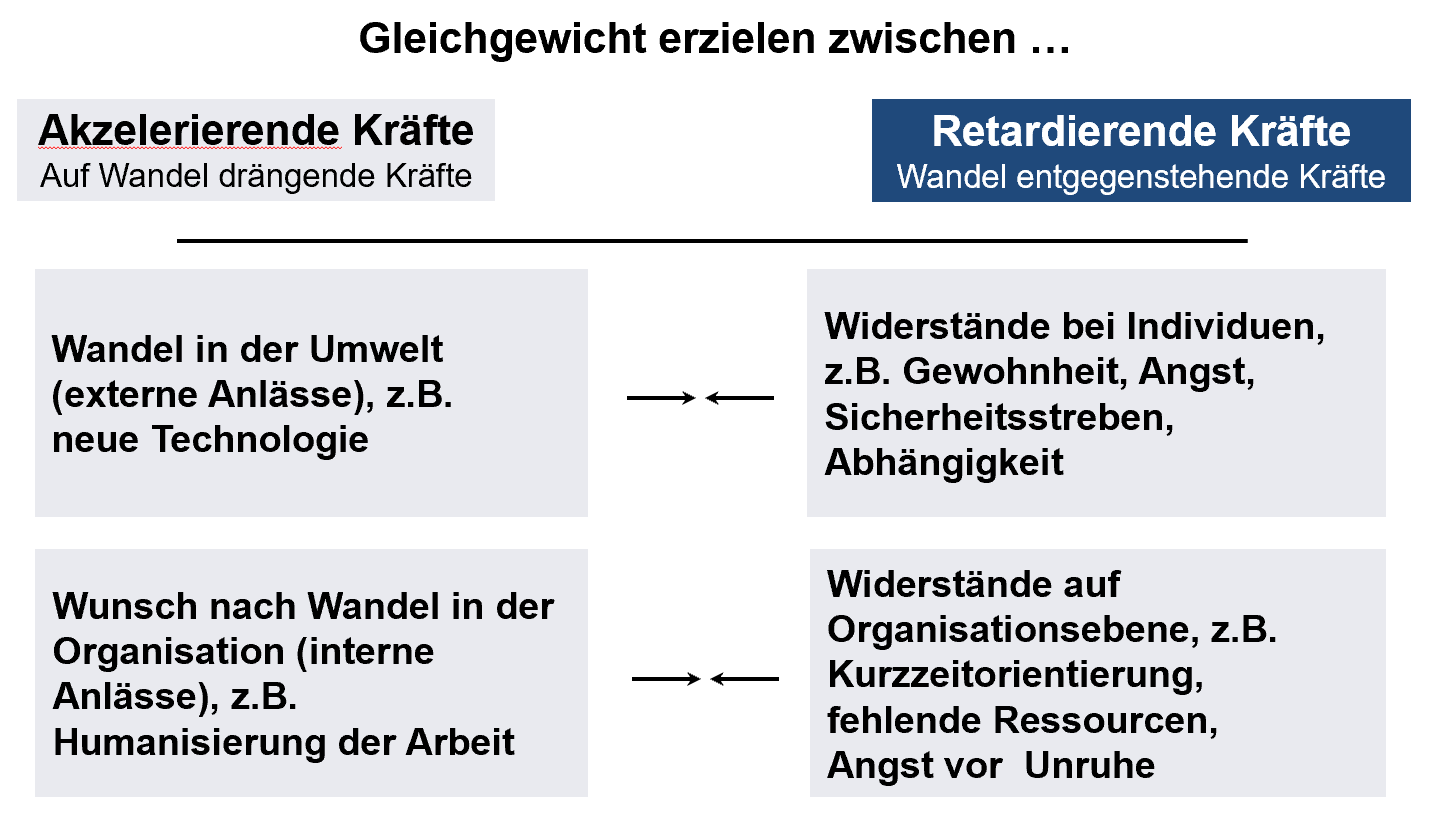
\includegraphics[width=15cm]{kurtlewins1}
		\item Drei Phasen von Veränderungsprozessen
			\begin{itemize}
			\item 1. Auftauen (Motivation für Veränderung wecken)
			\item 2. Verändern (Neue Reaktionsweise herausbilden)
			\item 3. Einfrieren (Stabilisierung und Integration der Änderung)
			\end{itemize}
		\item Erfolgsfaktorenmodell des Change Managaments
			\begin{itemize}
			\item 1. Orientierung (Feste Struktur, Versorgung mit Informationen)
			\item 2. Startmotivation (Akzeptanz + Konflikt = Entwicklung)
			\item 3. Prozessmotivation (Motivation von längerer Dauer, Prozess selbst Befriedigung)
			\item 4. Zielmotivation (VIE-Theorie)
			\end{itemize}
		\end{itemize}
	\end{itemize}

\end{itemize}

\section{Analyse von Geschäftsprozessen}
\subsection{Analyse und Optimierung von Geschäftsprozessen}
\begin{itemize}
\item Projektablauf:
\item[] 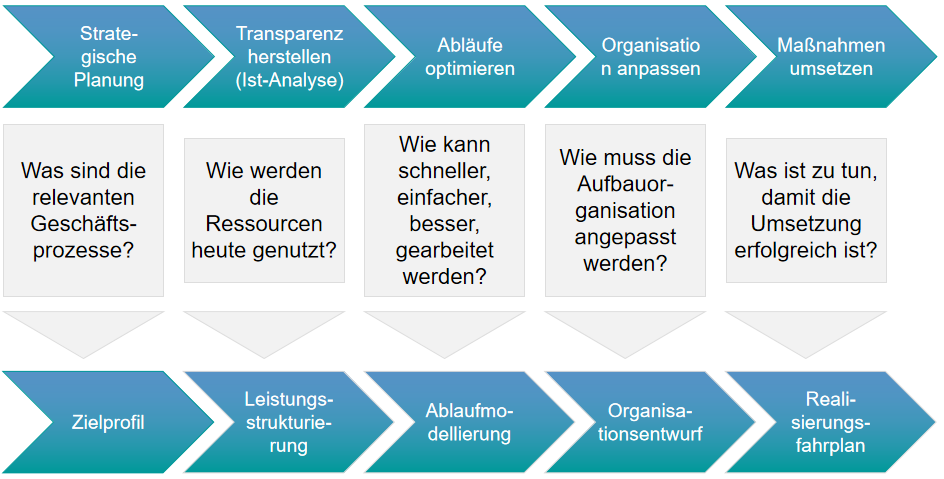
\includegraphics[width=15cm]{projektablauf}


\item Strategische Planung
	\begin{itemize}
	\item \textbf{1.} Führungskräftebefragung (Lösungen, Stärken, Schwächen,..)
	\item \textbf{2.} Kundeninterviews (Anforderungen, Schwachstellen)
	\item \textbf{3.} Wettbewerbsanalyse (qualitative/quantitative Vergleiche)
	\item \textbf{4.} Prozessauswahl (Mögliche Prozesse / Kriterien)
	\end{itemize}
	
\item Transparenz herstellen (Ist-Analyse)
	\begin{itemize}
	\item \textbf{1.} Ablaufanalyse (Ermittlung und Darstellung)
	\item \textbf{2.} Kapazitätserhebung (Ermittlung Mengengerüst)
	\item \textbf{3.} SOLL-Profil-Ermittlung (Festlegung der Zielstrukturen) 
	\item \textbf{4.} Ableitung Verbesserungspotential (Zeit, Menge, Kosten, Qualität)
	\end{itemize}
	
\item Abläufe optimieren
	\begin{itemize}
	\item Ideen aus Lean Management und BPR für Schwachstellenanalyse
	\item Ablaufoptimierung (Reduzierung Durchlaufzeit, Verringerung Komplexität, Erhöhung Auslastung)
	\item Hebel zur Prozessneugestaltung
	\item[] 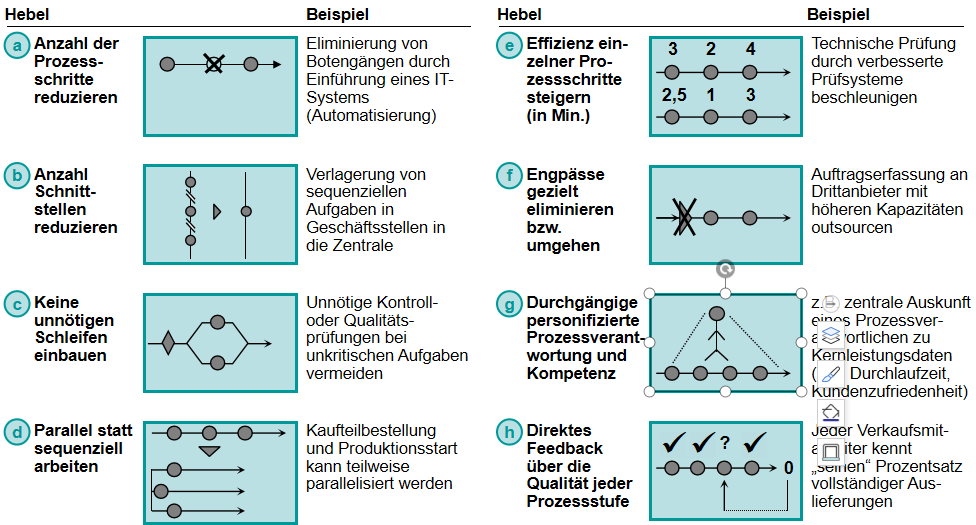
\includegraphics[width=15cm]{hebel}
	\end{itemize}

\item Organisation anpassen
	\begin{itemize}
	\item Identifizieren von Prozessblockern (Überschneidungen, Intransparenz,..)
	\item[$\rightarrow$] Abgegrenzte Verantwortung, wenig Schnittstellen, flache Hierarchie
	\end{itemize}
	
\item Maßnahmen umsetzen
	\begin{itemize}
	\item Ideen 
	\item Bewertung der Ideen (Einteilung, Zusammenfassen, ..)
	\item Maßnahmen (Ausarbeitung, Projekte,..)
	\end{itemize}
\end{itemize}

\subsection{Fallbeispiel Dunlop}

\section{Simulation und IT-Unterstützung von Geschäftsprozessen}
\subsection{Einordnung, Zweck und typische Fragestellungen}
\begin{itemize}
\item Simulation
	\begin{itemize}
	\item Vorbereiten, Durchführen und Auswerten gezielter Experimente
	\item Übertragung der Ergebnisse auf die Wirklichkeit
	\item Ziele:
		\begin{itemize}
		\item Verbesserung Betriebsabläufe
		\item Vermeidung kostentreibender Experimente
		\item Bewertung verschiedener Abläufe
		\end{itemize}
	\item Einsatzszenarien: 
		\begin{itemize}
		\item Ressourcen- und Kapazitätsplanung
		\item Prozess- und Arbeitsumgebungsoptimierung
		\item  Ermittlung von mengen- und kostenabhängigen Ergebnissen
		\end{itemize}
	\item Typische Ergebnisse:
		\begin{itemize}
		\item Durchschnittliche Durchlaufzeit
		\item Auslastung der beteiligten Ressourcen 
		\item Ermittlung der Kosten
		\item Liegezeiten der Vorgänge
		\end{itemize}
	\item Simulation als Entscheidungsgrundlage
	\end{itemize}
\end{itemize}

\subsection{Zusätzliche Aufgaben und Verteilungsannahmen in GP}
\begin{itemize}
\item  Beispiel Prozesssimulation mit eEPKs
\item[] 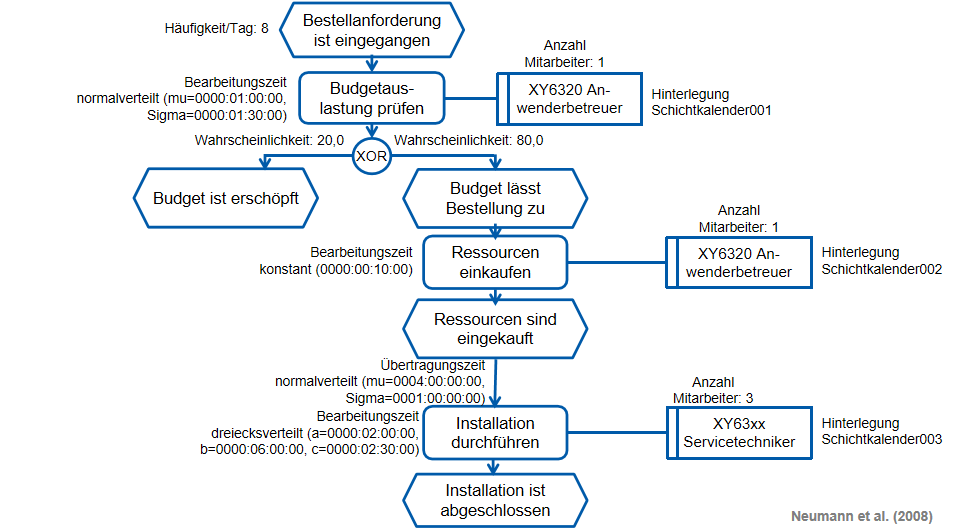
\includegraphics[width=15cm]{simeepk} 
\item Überblick simulationsrelevanter Aufgaben
\item[] 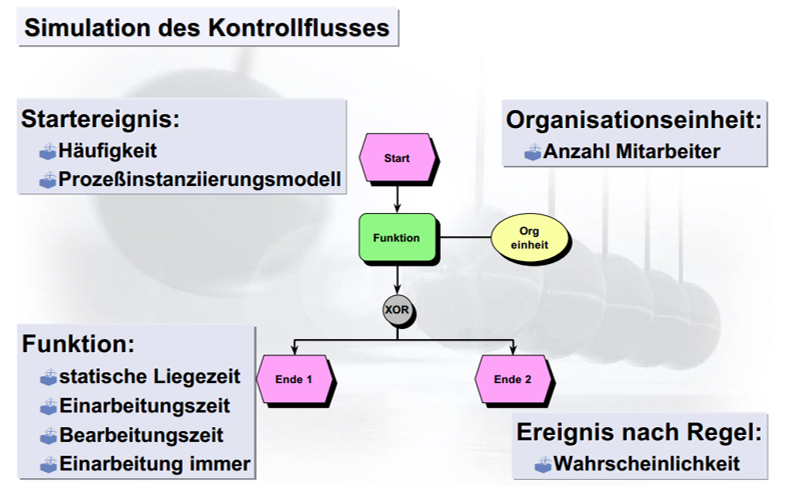
\includegraphics[width=15cm]{simaufgaben} 
\item Prozesssimulation: (Ergänzung des eEPKs)
	\begin{itemize}
	\item Rollen:
		\begin{itemize}
		\item Art der Ressource 
		\item Zeitliche Verfügbarkeit der Ressourcen
		\item Kosten der Ressourcen pro Zeiteinheit
		\end{itemize}
	\item Ereignisse:
		\begin{itemize}
		\item Anzahl und Art der simulierenden Eingangsereignisse
		\item Wann und in welchem Abstand treten Eingangsereignisse auf
		\end{itemize}
	\item Aktivitäten:
		\begin{itemize}
		\item Abschätzung der Dauer
		\item Zuordnung der ausführenden Rolle
		\item Anfallende Kosten
		\end{itemize}
	\item Verzweigungen:
		\begin{itemize}
		\item Wahrscheinlichkeitsfunktion der Verzweigungen
		\end{itemize}
	\end{itemize}
	
\item Statistik:
	\begin{itemize}
	\item Wahrscheinlichkeiten basierend aufgrund alter Daten
	\item Verschiedene Verteilungsfunktionen
	\end{itemize}

\end{itemize}

\subsection{Zentrale Simulationsanalysen}
\begin{itemize}
\item Pfadanalyse:
	\begin{itemize}
	\item Bewertung von GP-Modellen ohne Berücksichtigung der Arbeitsumgebung
	\item Basis dafür ist ein Prozessmodell mit allen zugehörigen Subprozessen
	\item Ergebnis: prozess- und pfadbezogene Ergebnisse (durchschnittliche Zeiten und Kosten)
	\item Bewertung der Pfade anhang ihrer Auftrittswahrscheinlichkeiten
	\item[] 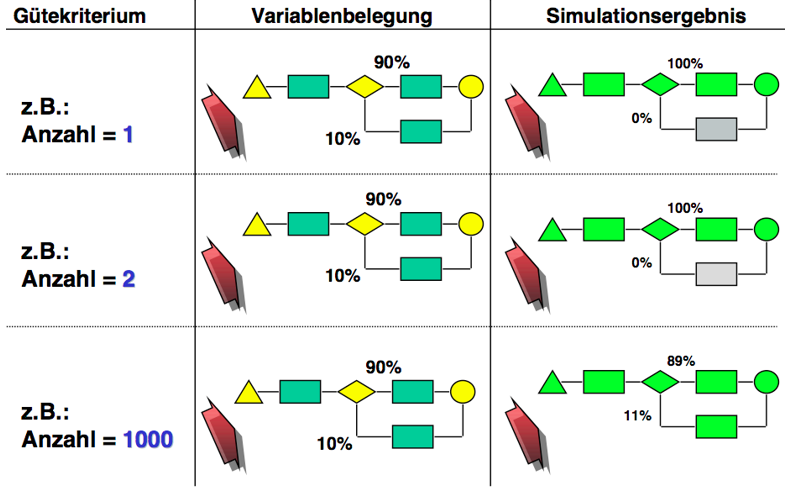
\includegraphics[width=15cm]{pfadstat}
	\end{itemize}

\item Belastungsanalyse
	\begin{itemize}
	\item Simuliert GP unter Berücksichtigung der zugehörigen Arbeitsumgebung
	\item "Ausführung" der Aktivitäten von ihren Bearbeitern
	\item Dadurch Aussagen zu Belastungen möglich
	\item Ermöglicht Ausführung einer Personalbedarfsplanung
	\end{itemize}

\item Auslastungsanalyse
	\begin{itemize}
	\item Unterstützt die Analyse des dynamischen Verhaltens einer Organisation
	\item Simulation von Wartezeiten auf Basis eines Warteschlangenmodells
	\item Beschreibung der stochastischen Häufigkeitsraten (mithilfe von Prozesskalendern)
	\item Erstellung von Auslastungsprofilen von Stellen
	\item Ermittlung von Engpässen und Leerzeiten
	\end{itemize}

\item Vor- und Nachteile von Simulation
	\begin{itemize}
	\item[+] Quantitative Auswerung von komplexen Prozessmodellen
	\item[+] "Was-Wäre-Wenn Szenarien"
	\item[+] Identifikation von Schwachstellen
	\item[-] Qualität stark abhängig von der Qualität der Eingangsdaten
	\item[-] Realitätsnähe
	\item[-] Definition von Störgrößen besonders problematisch	
	
	\end{itemize}

\end{itemize}
\pagebreak

\subsection{IT-Unterstützung}
\begin{itemize}
\item Einsatzmöglichkeiten von IT zur Unterstützung des GPM
\item[] 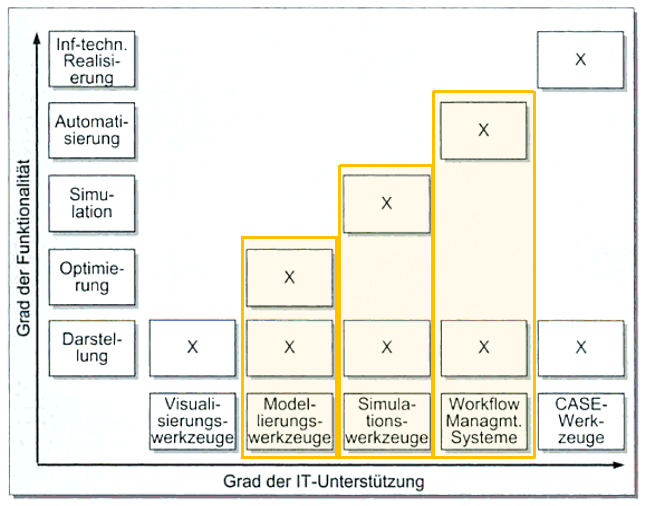
\includegraphics[width=15cm]{itsup}
\item Workflow-Management-Systeme (WFMS)
	\begin{itemize}
	\item Software-System zur Steuerung des Arbeitsflusses zwischen beteiligten Stellen
	\item geeignet für stark strukturierte, automatisierbare und regelmäßig stattfindende Prozesse 
	\item[] 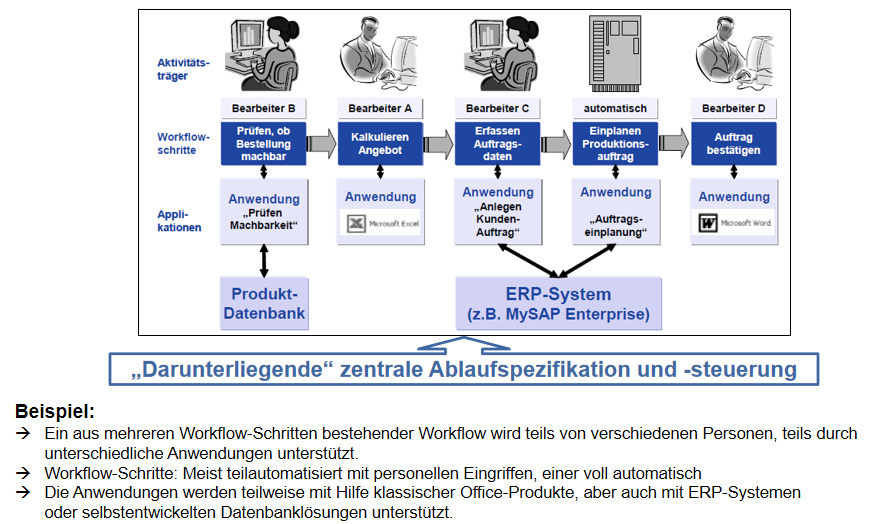
\includegraphics[width=15cm]{wfms}
	\end{itemize}
\end{itemize}

\end{document}





		